\documentclass[a4paper,12pt]{article}
\usepackage{graphicx}
\usepackage{caption}

\begin{document}

\title{Architectural Patterns and Styles - Notes}
\author{Priscilla Madigoe}
\date{08 March 2016}
\maketitle
 
\section{Architectural Patterns}

\subsection{Introduction}
Often times source code needs to be organised so that clear roles, responsibilities and relationships of different modules of the code can be well defined. Architectural patterns help in making this possible and numerous types will be discussed in this section. Using these patterns, code becomes easier to maintain, manage and visualise. They also make understanding of how each component works in a system easier. They are reusable solutions to a commonly occuring problems within a given context in Software Architecture.

\subsection{Types of Architectural Patterns}

\begin{itemize}
\item Layered Pattern
\item Client-server
\item Microkernel
\item Master-slave
\item Pipe-filter
\item Hierarchical
\item Model View Controller
\item Blackboard Pattern
\end{itemize}

\subsection{Architectural Patterns Proposed for PAPERS}


\subsubsection{Model View Controller}

\begin{itemize}
\item{Overview}

In the Model-View-Controller Pattern, an interactive application is divided into three parts: the Model is an object representing and storing the data and activities, the View displays information to the user and the Controller offers a way to change the state of the Model. To implement this patten for the system, the Python Django Framework will be used.

\begin{minipage}{\linewidth} 
\centering
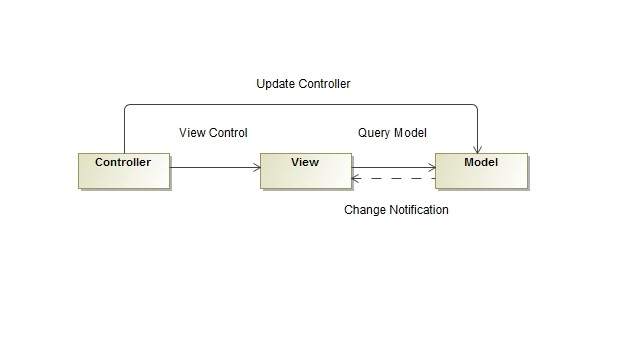
\includegraphics[width=4in]{C:/Users/Priscilla/Documents/GitHub/Charlie/Diagrams/ArchitecturalPatterns/ModelViewController.jpg}
\captionof{figure}{Model View Controller Pattern}
\end{minipage}

\item{Motivation}
\newline
Separation of responsibilities is useful because functions can work normally when certain subsystems are changed. The Model View Controller makes this a possibility and hence it is chosen for use in this context. 

\item{Components of the Model View Controller Pattern}
\begin{enumerate}
\item{Model}
\newline
The Django Framework provides a Model functionality that handles the creation and storage of data in a relational databse that will contain essential fields and behaviours of the data stored for the system.
\newline

\item{View}

Normally, the View would be the HTML page or the Android Graphic User Interface, or GUI that displays data from the relational databse to the user for interaction purposes. However, Django implements the View as a "Python callback function for a particular  URL, because that callback function describes which data is presented" to the user. Thus the View would be both the User Interface and Django's  implementation of the View for the system.
\newline
\item{Controller}

The Django Framework itself will be the Controller as it will provide appropriate functionality for data manipulation. It will be used along with the REST, or Representational State Transfer API to retrieve data from the Android and the Web Interface.

\end{enumerate}
\end{itemize}

\subsubsection{Layered Pattern}
\begin{itemize}
\item{Overview}
\newline
The Layered Pattern assists in structuring applications that can be decomposed into subtasks. Each subtask provides services to the layer above it and services in that layer are implemented using those from the layer below it.
\newline
\begin{minipage}{\linewidth} 
\centering
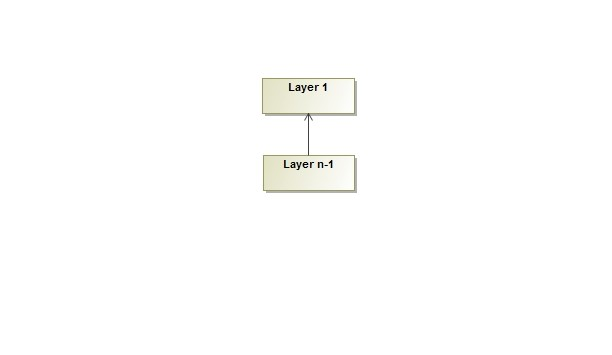
\includegraphics[width=4in]{C:/Users/Priscilla/Documents/GitHub/Charlie/Diagrams/ArchitecturalPatterns/LayeredPattern.jpg}
\captionof{figure}{Layered Pattern}
\end{minipage}
\item{Motivation}
\newline
A system typically consists of subsystems that have a certain functionality. These functions need to be placed in layers so that their services can be used by other layers and a change in behaviour of one layer does not affect the layers below it. This assists in developing different layers independently. 

\item{Components of the Layered Pattern}
\newline
This pattern will be used to separate the internal functions within each subsystem and each function will be placed in a layer. It will be used to structure the Model View Controller Pattern described above to provide additional decoupling and structure to the system.
\newline

\end{itemize}


\subsubsection{Master-Slave}
\begin{itemize}
\item{Overview}
\newline
The Master-slave Pattern can be described as  a model where one process (Master) has unidirectional control over one or more processes that are known as Slaves. 
\newline
\begin{minipage}{\linewidth} 
\centering
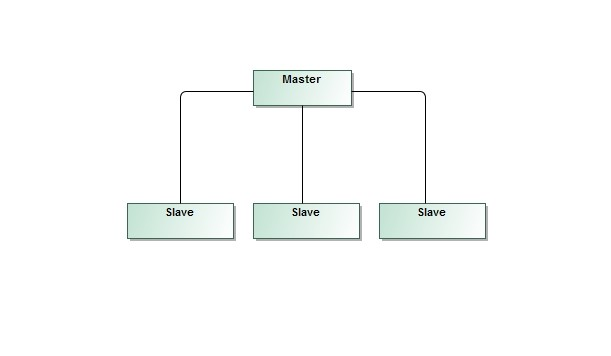
\includegraphics[width=4in]{C:/Users/Priscilla/Documents/GitHub/Charlie/Diagrams/ArchitecturalPatterns/MasterSlave.jpg}
\captionof{figure}{Master Slave}
\end{minipage}
\item{Motivation}
\newline
An interactive application typically consist of multiple users that use it at different rates. These users make requests that usually expect a response to either use the data or edit it in some way and thus is imperative for the application have an ability to collect user information simultaneously.

\item{Components of the Master-Slave Pattern}
\newline
This pattern will be used to make the system concurrent, i.e to enable multiple users to use it simultaneously and continuously at different rates.
\begin{itemize}
\item{Master} 
\newline
The Master will be the server that will respond to each request it receives from the Slave using the system, and will also provide instructions to these Slaves.
\item{Slaves}
\newline 
The Slaves will be the clients connecting to the server and will  send requests concurrently to achieve a certain goal.
\end{itemize}
\end{itemize}

\subsection{Other Patterns}
\subsubsection{Client Server Pattern}

\begin{itemize}

\item Client Application provides access to humans, or systems (Fritz, 2012)
\item Requests are typically handled in separate threads on the server.
\item Inter-process communication causes overhead.
\item Requests and data have to be transformed because they have different representation in Server and Client.
\end{itemize}

\subsubsection{Microkernel}
\begin{itemize}
\item Used for applications that must adapt to changing system requirements.
\item This pattern provides minimal functionality (Internal Servers) as a building block and customizable components that can be adapted accordingly (External Servers).
\item It provides an Adapter that provides a single access point (Fritz, 2012)
\item It offers a more complex process management if not provided by architecture (Fritz, 2012)
\end{itemize}

\subsubsection{Pipes and Filters}
\begin{itemize}
\item Consists of Pipes and Filters:
\begin{itemize}
\item Pipe - Input and Output
\item Filters - Stateless sevices or pure functions.
\end{itemize}
\item Assemble higher-level stateless services from lower level ones (Fritz, 2012)
\item It is not used because it is difficult to use for interactive processes such as Web Applications.

\end{itemize}

\subsubsection{Hierarchical}
\begin{itemize}
\item It is a recursive containment hierarchy (Fritz, 2012)
\item It is not used due to its lack of flexibility.
\end{itemize}

\subsubsection{Blackboard Pattern}
\begin{itemize}
\item Blackboard repository hosts problem specification and current state of solution (Fritz, 2012)
\item It is typically used where deterministic solutions are unavailable.
\item It is not used because it requires complex synchronization and access control techniques. 
\end{itemize}

\end{document}